\section{Diseño experimental}

\subsection{Sobreajuste y poda}


texto



En la figura~\ref{fig:3a} se muestra la grafica el número de hojas en función de la función de poda.

\begin{figure}
  \centering
  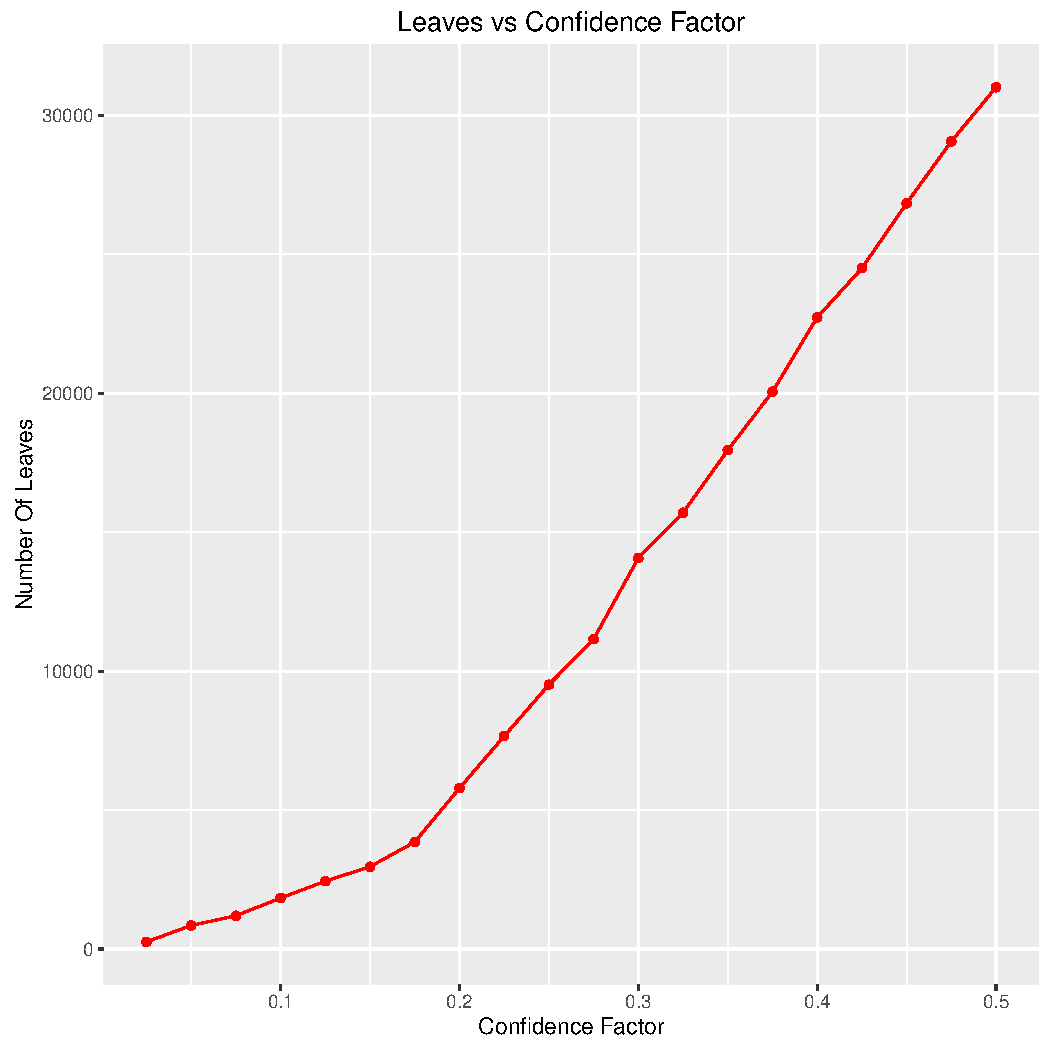
\includegraphics[width = 8cm]{3a.pdf}
  \caption{Number of leaves vs Confidence factor}
  \label{fig:3a}
\end{figure}

En la figura~\ref{fig:3b} se muestra la grafica el performance en función de la función de poda.

\begin{figure}
  \centering
  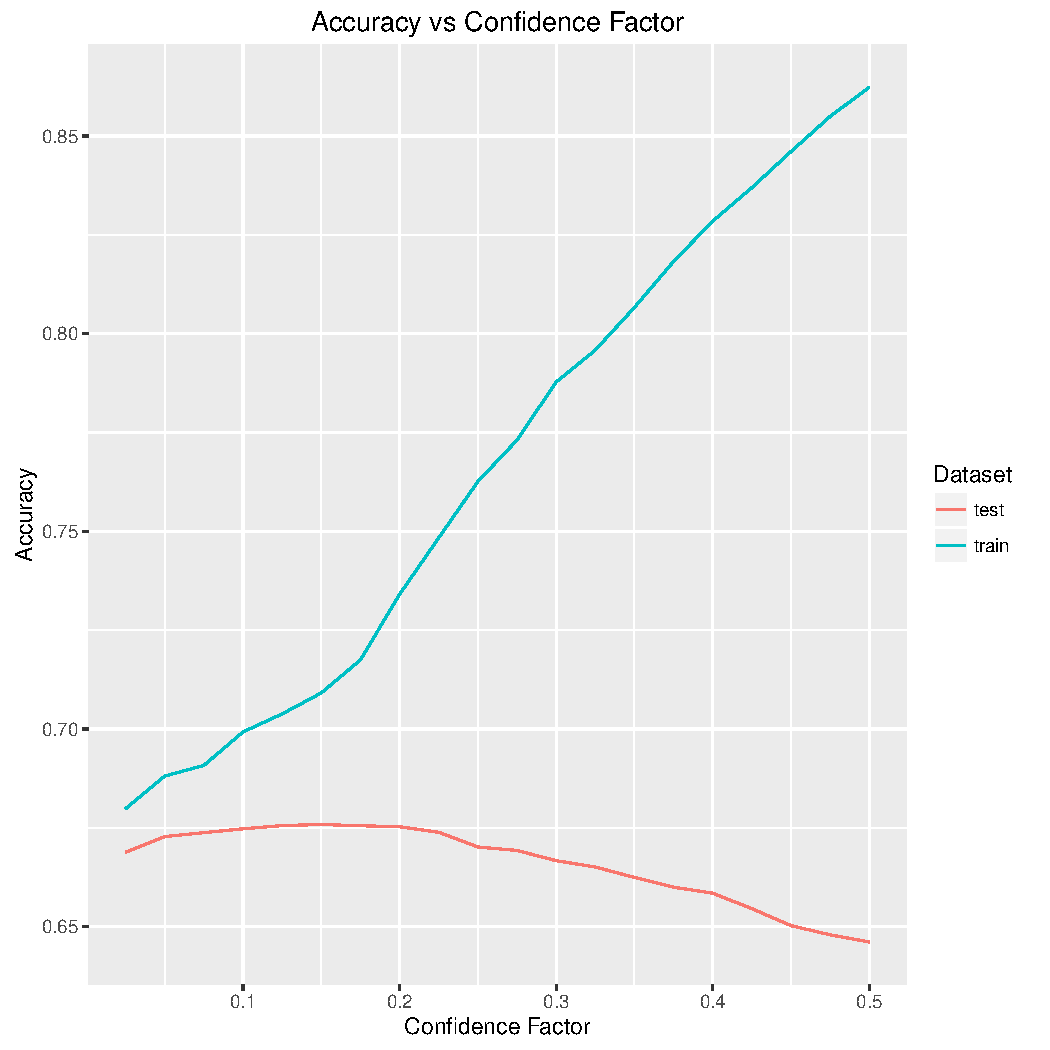
\includegraphics[width = 8cm]{3b.pdf}
  \caption{Accuracy vs Confidence factor}
  \label{fig:3b}
\end{figure}


En la figura~\ref{fig:3c} se muestra la grafica de la curva ROC para el mejor árbol,

\begin{figure}
  \centering
  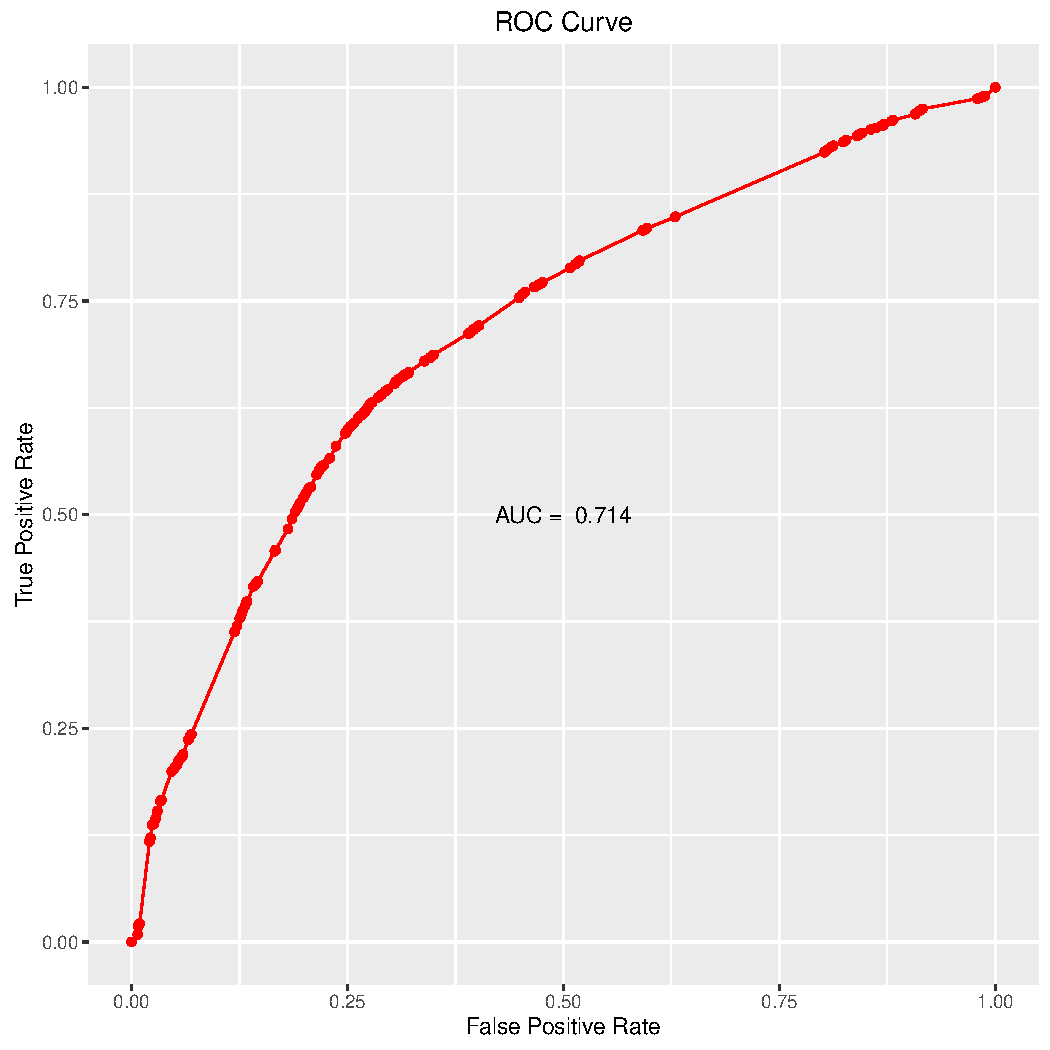
\includegraphics[width = 8cm]{3c.pdf}
  \caption{Curva ROC mejor árbol}
  \label{fig:3c}
\end{figure}


